\documentclass{article}
\usepackage[T1]{fontenc}
\usepackage{lmodern}
\usepackage{graphicx}
\usepackage{amsmath,amssymb}
\usepackage[a4paper,margin=2cm]{geometry}
\usepackage[absolute,overlay]{textpos}
\setlength{\TPHorizModule}{1mm}
\setlength{\TPVertModule}{1mm}
\usepackage[indonesian]{babel}
\usepackage{hyperref}
\setlength{\emergencystretch}{2em}
% unit: Halaman 51

\begin{document}

% === Halaman 51 (llm) ===

\section*{Ekstraksi Pesan dari $Stego\text{-}image$}

\begin{itemize}
    \item Bit-bit pesan yang disembunyikan di dalam citra harus dapat diekstraksi kembali.
    \item Caranya adalah dengan membaca $byte\text{-}byte$ di dalam citra, mengambil LSB-nya, dan merangkainya kembali menjadi bit-bit pesan.
    \item Contoh: Misalkan $stego\text{-}object$ adalah sbb
\end{itemize}

\vspace{5mm}

Ekstrak bit-bit LSB: $\mathbf{1110010111}$

% deskripsi: Contoh representasi biner dari stego-object dengan bit LSB yang diwarnai biru untuk menunjukkan proses ekstraksi.
% bbox normalisasi: [0.1060, 0.6020, 0.6820, 0.7150]
\begin{textblock*}{120.96mm}(22.26mm,178.79mm)
\noindent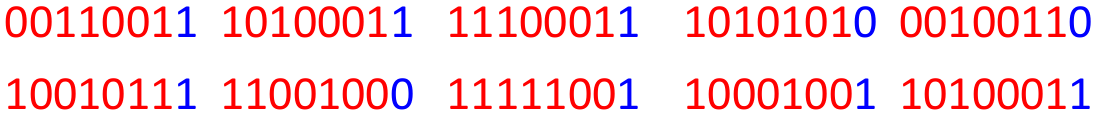
\includegraphics[width=120.96mm,height=33.56mm]{../../images/llm/page_051_img_01.png}%
\end{textblock*}

\end{document}
